\documentclass{ieeeaccess}
\usepackage{cite}
\usepackage{amsmath,amssymb,amsfonts}
\usepackage{algorithmic}
\usepackage{graphicx}
\usepackage{textcomp}
\usepackage{booktabs}
\usepackage{multirow}
\usepackage{url}
\usepackage{hyperref}
\usepackage{xcolor}
\usepackage{array}

\graphicspath{{../figures/}}

\begin{document}
\history{Date of publication xxxx 00, 0000, date of current version xxxx 00, 0000.}
% \doi{} % Assigned by IEEE upon acceptance

\title{Unsupervised Anomaly Detection in Hospital Financial Statements: A Multi-Algorithm Consensus Approach with Explainable AI}

\author{
\uppercase{Yongjun Kim}\authorrefmark{1},
ORCID: 0000-0003-4234-4883
and
\uppercase{Eun Jung Sun}\authorrefmark{2}
(Corresponding Author: Eun Jung Sun)}

\address[1]{Department of Software, Ajou University, Suwon 16499, South Korea (e-mail: yjkim0123@ajou.ac.kr)}
\address[2]{Department of Accounting, College of Economics and Business Administration, Hannam University, Daejeon 34430, South Korea (e-mail: belle@hnu.kr)}

\tfootnote{This research received no external funding.}

\markboth
{Kim and Sun: Unsupervised Anomaly Detection in Hospital Financial Statements}
{Kim and Sun: Unsupervised Anomaly Detection in Hospital Financial Statements}

\begin{abstract}
Monitoring the financial health of hospitals is critical for healthcare sustainability, yet traditional approaches rely on supervised learning methods that require labeled datasets---an assumption rarely met in practice. This study proposes a multi-algorithm consensus framework for unsupervised anomaly detection in hospital financial statements. Using a balanced panel of 165 Korean general and tertiary hospitals over five fiscal years (2019--2023, $N = 827$), we apply five complementary unsupervised algorithms: Isolation Forest, Local Outlier Factor, One-Class SVM, DBSCAN, and an autoencoder based on reconstruction error. A consensus mechanism identifies ``strong anomalies'' as observations flagged by three or more algorithms, yielding 57 consensus anomalies (6.9\%). Mann-Whitney U tests reveal that consensus anomalies exhibit significantly higher labor cost ratios ($p < 0.001$), administrative cost ratios ($p < 0.001$), and subsidy dependence ($p < 0.001$) compared to normal hospitals. Temporal analysis shows anomaly rates increasing from 6.1\% in 2019 to 8.5\% in 2023, suggesting growing financial heterogeneity in the post-COVID era. SHAP-based explainability analysis on the Isolation Forest identifies hospital ownership type, subsidy ratio, and administrative costs as the primary drivers of anomaly scores. Notably, only 47.4\% of consensus anomalies overlap with accounting-deficit hospitals ($\chi^2 = 0.67$, $p = 0.414$), indicating that unsupervised anomaly detection captures structurally unusual financial patterns beyond simple profitability, offering a complementary surveillance tool for healthcare regulators.
\end{abstract}

\begin{keywords}
Anomaly detection, hospital finance, unsupervised learning, consensus approach, Isolation Forest, SHAP, explainable AI, healthcare management
\end{keywords}

\titlepgskip=-15pt

\maketitle

% ══════════════════════════════════════════════════════════════════
\section{Introduction}
\label{sec:intro}
% ══════════════════════════════════════════════════════════════════

\IEEEPARstart{H}{ospital} financial sustainability has emerged as a pressing concern worldwide, particularly in the wake of the COVID-19 pandemic that disrupted healthcare delivery and revenue streams~\cite{cutler2020impact, khullar2020covid}. In South Korea, where general and tertiary hospitals constitute the backbone of the healthcare system, monitoring financial health is essential for preventing hospital closures and ensuring equitable access to care~\cite{yeo2018closure, lee2024covid}.

Conventional approaches to hospital financial surveillance typically rely on ratio analysis or supervised machine learning models that predict binary outcomes such as financial distress or deficit~\cite{bai2016analysis, oner2024hospital}. While effective when labeled training data are available, supervised methods face two fundamental limitations in this domain. First, defining ``financial distress'' is inherently subjective---a hospital reporting a net loss in a single year may be strategically investing rather than experiencing genuine distress. Second, labeled datasets are scarce; regulatory agencies rarely maintain curated databases of financially anomalous hospitals, and the class boundaries between distressed and healthy institutions are often ambiguous~\cite{kim2024financial}.

Unsupervised anomaly detection offers a compelling alternative. Rather than requiring predefined labels, these methods identify observations that deviate substantially from the expected distribution of data, flagging institutions whose financial profiles are structurally unusual~\cite{chandola2009anomaly, pang2021deep}. This label-free approach is particularly valuable for financial surveillance, where the goal is not necessarily to predict bankruptcy but to identify hospitals warranting closer regulatory scrutiny.

However, unsupervised methods suffer from a well-known limitation: different algorithms make different assumptions about data structure and consequently flag different subsets of observations~\cite{goldstein2016comparative, domingues2018comparative}. An Isolation Forest excels at identifying globally isolated points in feature space~\cite{liu2008isolation}, while the Local Outlier Factor captures local density deviations~\cite{breunig2000lof}, and One-Class SVM delineates a boundary around the support of the data distribution~\cite{scholkopf2001estimating}. No single algorithm is universally optimal.

To address this challenge, we propose a \textbf{multi-algorithm consensus framework} that combines five complementary unsupervised anomaly detection algorithms and identifies ``strong anomalies'' as observations flagged by three or more methods. This ensemble approach reduces the false-positive rate inherent in any single algorithm while capturing diverse notions of abnormality. We further enhance interpretability by applying SHAP (SHapley Additive exPlanations)~\cite{lundberg2017unified} to explain the drivers of anomaly scores, bridging the gap between black-box detection and actionable insight.

Our contributions are as follows:
\begin{enumerate}
    \item We construct a comprehensive framework applying five unsupervised anomaly detection algorithms---Isolation Forest, LOF, One-Class SVM, DBSCAN, and autoencoder---to hospital financial data and introduce a consensus mechanism for robust anomaly identification.
    \item We analyze a balanced panel of 165 Korean hospitals over 2019--2023, providing temporal insights spanning the pre-COVID, pandemic, and recovery periods.
    \item We apply SHAP-based explainability to the Isolation Forest model, identifying the financial and structural features that drive anomaly scores.
    \item We compare unsupervised anomalies with supervised deficit labels, demonstrating that the two approaches capture complementary dimensions of financial risk.
\end{enumerate}

The remainder of this paper is organized as follows. Section~\ref{sec:related} reviews related work. Section~\ref{sec:method} describes the data, algorithms, and analytical framework. Section~\ref{sec:results} presents the experimental results. Section~\ref{sec:casestudy} provides a detailed case study profiling consensus anomalies. Section~\ref{sec:discussion} discusses implications, validation, and limitations. Section~\ref{sec:conclusion} concludes with future directions.

% ══════════════════════════════════════════════════════════════════
\section{Related Work}
\label{sec:related}
% ══════════════════════════════════════════════════════════════════

\subsection{Financial Anomaly Detection}
\label{subsec:financial_anomaly}
Anomaly detection in financial data has been extensively studied across domains including fraud detection, credit scoring, and financial statement analysis. Ngai et al.~\cite{ngai2011application} provided an early classification framework for data mining techniques in financial fraud detection, reviewing 49 journal articles and categorizing methods by fraud type (bank fraud, insurance fraud, securities and commodity fraud, and others). Ahmed et al.~\cite{ahmed2016survey} extended this line of inquiry with a survey of anomaly detection techniques specifically tailored to the financial domain, distinguishing between supervised, semi-supervised, and unsupervised approaches and highlighting the growing importance of ensemble methods. More recently, Hilal et al.~\cite{hilal2022financial} presented a comprehensive review of anomaly detection techniques for financial fraud, covering both traditional statistical methods and modern deep learning approaches, and identifying semi-supervised and unsupervised methods as particularly promising directions given the chronic scarcity of labeled financial data.

Chandola et al.~\cite{chandola2009anomaly} provided a comprehensive taxonomy of anomaly detection techniques, categorizing methods into statistical, proximity-based, and machine-learning-based approaches. Pang et al.~\cite{pang2021deep} surveyed deep learning methods for anomaly detection, noting the trade-off between detection power and interpretability. In the financial domain, unsupervised methods are particularly attractive because labeled fraud or distress data are rare and the boundary between normal and anomalous behavior is often unclear~\cite{aggarwal2017outlier}. West and Bhattacharya~\cite{west2016intelligent} reviewed intelligent financial fraud detection systems, emphasizing that the class imbalance problem in financial datasets makes supervised approaches prone to high false-negative rates, further motivating unsupervised alternatives.

Goldstein and Uchida~\cite{goldstein2016comparative} conducted a comparative evaluation of unsupervised anomaly detection algorithms on multivariate datasets, finding that no single method dominates across all scenarios. Similarly, Domingues et al.~\cite{domingues2018comparative} showed that algorithm performance varies substantially with data characteristics, motivating ensemble or consensus approaches. Ruff et al.~\cite{ruff2021unifying} provided a unifying theoretical framework for deep and shallow anomaly detection, showing that most methods can be understood through a common lens of learning representations that concentrate normal data, while isolating anomalies.

\subsection{Healthcare Financial Distress}
\label{subsec:healthcare_distress}
Research on hospital financial performance has a long history rooted in financial ratio analysis. Altman's~\cite{altman1968financial} seminal Z-score model, originally developed for manufacturing firms, introduced multiple discriminant analysis for bankruptcy prediction using five financial ratios. This model has been subsequently adapted to the healthcare sector. Lord et al.~\cite{lord2020predicting} applied a modified Altman Z-score to predict financial distress in U.S. nursing homes, using K-means clustering to classify facilities into distressed, at-risk, and healthy categories based on the Z-score distribution. Holmes et al.~\cite{holmes2017predicting} developed a financial distress index for rural hospitals in the United States, combining multiple financial indicators to predict both distress and closure risk, and identifying three key financial ratios---days cash on hand, equity financing ratio, and operating margin---as the strongest predictors.

Bai and Anderson~\cite{bai2016analysis} analyzed the financial performance of U.S. hospitals from 2006 to 2013 using operating margins and total margins, revealing significant variation by ownership type and geographic location. Langabeer et al.~\cite{langabeer2018predicting} used logistic regression to predict financial distress in acute care hospitals, finding that liquidity ratios and profitability measures were the most significant determinants. Enumah and Chang~\cite{holmes2021predictors} extended this work by examining predictors of financial distress among private U.S. hospitals, identifying case complexity and outpatient revenue proportion as potential intervention points. More recently, {\"O}ner and Ba{\c{s}}o{\u{g}}lu~\cite{oner2024hospital} applied machine learning methods---including Random Forest, XGBoost, and neural networks---to evaluate hospital financial distress, demonstrating that AI-based approaches can improve predictive accuracy over traditional ratio-based methods.

The COVID-19 pandemic catalyzed renewed interest in hospital financial vulnerability. Cutler~\cite{cutler2020impact} documented the pandemic's impact on U.S. healthcare finances, while Khullar et al.~\cite{khullar2020covid} specifically examined the financial health of U.S. hospitals during the pandemic. In Korea, Lee~\cite{lee2024covid} provided an observational study of the pandemic's differential impact on hospital financial performance according to hospital characteristics. Kim and Sun~\cite{kim2024financial} applied panel data analysis combined with supervised machine learning (Random Forest, Gradient Boosting) to predict financial distress in Korean general hospitals, identifying material cost ratio and year effects as key predictors. However, their supervised approach required binary deficit labels, limiting its applicability to surveillance scenarios where labels are unavailable.

\subsection{Unsupervised vs.\ Supervised Approaches and Ensemble Methods}
\label{subsec:unsupervised_vs_supervised}
The choice between supervised and unsupervised anomaly detection hinges fundamentally on the availability and reliability of ground truth labels~\cite{chandola2009anomaly}. In healthcare financial surveillance, ground truth is particularly problematic: financial distress is a continuous spectrum rather than a binary state, regulatory definitions of ``anomalous'' behavior vary across jurisdictions, and the base rate of truly anomalous hospitals is unknown. These challenges have motivated growing interest in unsupervised and semi-supervised approaches~\cite{ruff2021unifying}.

A key limitation of any single unsupervised algorithm is its dependence on specific assumptions about data structure. Zimek et al.~\cite{zimek2014ensembles} articulated the case for ensemble methods in unsupervised outlier detection, identifying challenges related to combining diverse detectors, defining appropriate combination functions, and evaluating ensemble performance in the absence of labels. Aggarwal and Sathe~\cite{aggarwal2017outlier_ensembles} provided a systematic treatment of outlier ensemble methods, showing that combining diverse base detectors through voting or averaging consistently improves detection robustness.

Despite these methodological advances, the application of unsupervised ensemble anomaly detection to healthcare financial data remains limited. Most studies in hospital finance employ supervised methods with binary labels (deficit/surplus or distressed/healthy), leaving a gap in the literature for frameworks that can identify structurally unusual financial patterns without predefined categories. Notably, the healthcare financial literature has not systematically examined whether combining multiple unsupervised detectors can yield more robust and interpretable results than individual algorithms applied in isolation.

Our work addresses this gap by applying a multi-algorithm consensus framework to hospital financial statements, combining five complementary unsupervised algorithms to achieve robust anomaly identification. Unlike prior approaches that rely on a single algorithm or use labeled outcomes as the gold standard, our consensus mechanism leverages the diversity among algorithms---each capturing different aspects of ``abnormality''---to produce a more reliable set of detected anomalies. The framework is deliberately algorithm-agnostic at the ensemble level: any combination of unsupervised detectors can be substituted, making it adaptable to different data characteristics and domain requirements.

\subsection{Explainable AI in Healthcare}
\label{subsec:xai}
The push for explainable AI (XAI) has grown in healthcare applications where model transparency is essential for clinical and regulatory trust~\cite{arrieta2020explainable}. SHAP values, grounded in cooperative game theory, provide consistent and locally accurate feature attributions~\cite{lundberg2017unified}. While SHAP has been widely applied to supervised healthcare models, its application to unsupervised anomaly detection---specifically explaining \textit{why} an observation is deemed anomalous---remains underexplored.

% ══════════════════════════════════════════════════════════════════
\section{Methodology}
\label{sec:method}
% ══════════════════════════════════════════════════════════════════

\subsection{Data Description}
\label{subsec:data}

We use publicly available financial statement data from the Korean Health Insurance Review and Assessment Service (HIRA), which mandates annual financial disclosures for all hospitals. The dataset comprises 165 general and tertiary hospitals with complete records across five fiscal years (2019--2023), forming a balanced panel of $N = 827$ hospital-year observations (two hospitals have minor missing observations handled during preprocessing).

Table~\ref{tab:features} describes the 11 features used for anomaly detection, derived from financial statement line items following the feature engineering approach of Kim and Sun~\cite{kim2024financial}.

\begin{table}[!t]
\centering
\caption{Feature Descriptions ($N = 827$)}
\label{tab:features}
\begin{tabular}{@{}lp{4.2cm}@{}}
\toprule
\textbf{Feature} & \textbf{Description} \\
\midrule
Material Cost Ratio & Material costs / Medical revenue \\
Labor Cost Ratio & Personnel costs / Medical revenue \\
Admin Cost Ratio & Administrative costs / Medical revenue \\
Debt Ratio & Total liabilities / Total assets \\
Subsidy Ratio & Donations / Total revenue \\
Log Revenue & Log of medical revenue \\
Log Beds & Log of number of beds \\
University Hospital & Binary: university-affiliated \\
Public Hospital & Binary: publicly owned \\
Tertiary Hospital & Binary: tertiary-care designation \\
Year & Fiscal year (0 = 2019, ..., 4 = 2023) \\
\bottomrule
\end{tabular}
\end{table}

All continuous features are standardized (zero mean, unit variance) prior to anomaly detection to ensure equitable weighting across algorithms sensitive to feature scale.

\subsection{Anomaly Detection Algorithms}
\label{subsec:algorithms}

We employ five unsupervised anomaly detection algorithms, each capturing a different notion of ``abnormality.''

\subsubsection{Isolation Forest (IF)}
The Isolation Forest~\cite{liu2008isolation, liu2012isolation} detects anomalies by recursively partitioning the feature space through random splits. Anomalous observations, being isolated in feature space, require fewer splits to separate from the rest, resulting in shorter average path lengths in the ensemble of isolation trees. We use 200 trees with a contamination parameter of 0.1.

\subsubsection{Local Outlier Factor (LOF)}
LOF~\cite{breunig2000lof} computes the local density of each observation relative to its $k$ nearest neighbors. Points in sparser regions receive higher LOF scores. We set $k = 20$ and contamination = 0.1.

\subsubsection{One-Class SVM (OCSVM)}
One-Class SVM~\cite{scholkopf2001estimating} learns a decision boundary that encloses the majority of the data in a kernel-induced feature space. Points falling outside the boundary are classified as anomalies. We use an RBF kernel with $\nu = 0.1$.

\subsubsection{DBSCAN}
DBSCAN~\cite{ester1996density} is a density-based clustering algorithm that labels points in low-density regions as noise (anomalies). We automatically tune the $\varepsilon$ parameter using the 90th percentile of the $k$-distance graph ($k = 5$), yielding $\varepsilon = 1.755$, which identified 7 clusters with noise points as anomalies.

\subsubsection{Autoencoder (AE)}
We implement a bottleneck autoencoder using a multi-layer perceptron with architecture $11 \rightarrow 8 \rightarrow 4 \rightarrow 8 \rightarrow 11$, trained to reconstruct the input features~\cite{hinton2006reducing}. Observations with high reconstruction error (above the 90th percentile) are flagged as anomalies, as they deviate from patterns learned from the majority of the data.

\subsection{Consensus Anomaly Framework}
\label{subsec:consensus}

Each algorithm independently produces a binary anomaly label for each observation. We define the \textbf{consensus anomaly score} as the number of algorithms flagging an observation:
\begin{equation}
    C_i = \sum_{a=1}^{5} \mathbb{1}[\text{Algorithm}_a(x_i) = \text{anomaly}]
\end{equation}
An observation is classified as a \textbf{consensus anomaly} if $C_i \geq 3$, i.e., the majority of algorithms agree. This threshold balances sensitivity and specificity: requiring unanimity ($C_i = 5$) would be overly conservative, while $C_i \geq 2$ would include many marginal cases.

\subsection{Explainability via SHAP}
\label{subsec:shap}

We apply TreeSHAP~\cite{lundberg2017unified} to the Isolation Forest model to compute feature-level contributions to each observation's anomaly score. SHAP values decompose the model output into additive feature contributions:
\begin{equation}
    f(x) = \phi_0 + \sum_{j=1}^{p} \phi_j
\end{equation}
where $\phi_j$ is the SHAP value for feature $j$ and $\phi_0$ is the base value. The mean absolute SHAP value $\overline{|\phi_j|}$ quantifies global feature importance.

\subsection{Statistical Analysis}
\label{subsec:stats}

We compare financial characteristics between consensus anomalies and normal observations using the Mann-Whitney U test~\cite{mann1947test}, a non-parametric test appropriate for potentially non-normal distributions. Pairwise agreement between algorithms is measured using the Jaccard similarity coefficient~\cite{jaccard1912distribution}. The association between anomaly status and accounting deficit is assessed using the chi-squared test.

% ══════════════════════════════════════════════════════════════════
\section{Results}
\label{sec:results}
% ══════════════════════════════════════════════════════════════════

\subsection{Per-Algorithm Anomaly Detection}
\label{subsec:per_algo}

Table~\ref{tab:algo_rates} presents the anomaly rates for each algorithm. Isolation Forest, LOF, One-Class SVM, and the autoencoder each flagged approximately 10\% of observations, consistent with the contamination parameter. DBSCAN, which does not use a contamination parameter but relies on density-based clustering, flagged 6.2\% as noise points, identifying 7 distinct clusters.

\begin{table}[!t]
\centering
\caption{Anomaly Detection Results by Algorithm}
\label{tab:algo_rates}
\begin{tabular}{@{}lcc@{}}
\toprule
\textbf{Algorithm} & \textbf{Anomalies} & \textbf{Rate (\%)} \\
\midrule
Isolation Forest & 83 & 10.0 \\
Local Outlier Factor & 83 & 10.0 \\
One-Class SVM & 84 & 10.2 \\
DBSCAN & 51 & 6.2 \\
Autoencoder & 83 & 10.0 \\
\midrule
\textbf{Consensus ($\geq$3)} & \textbf{57} & \textbf{6.9} \\
\bottomrule
\end{tabular}
\end{table}

\subsection{Algorithm Agreement}
\label{subsec:agreement}

Fig.~\ref{fig:consensus_heatmap} shows the pairwise Jaccard similarity between algorithms. The highest agreement is between One-Class SVM and the autoencoder (Jaccard = 0.505), followed by Isolation Forest and One-Class SVM (0.427) and OCSVM and DBSCAN (0.421). The lowest agreement is between Isolation Forest and LOF (0.239), indicating that these two methods capture substantially different aspects of abnormality.

\begin{figure}[!t]
\centering
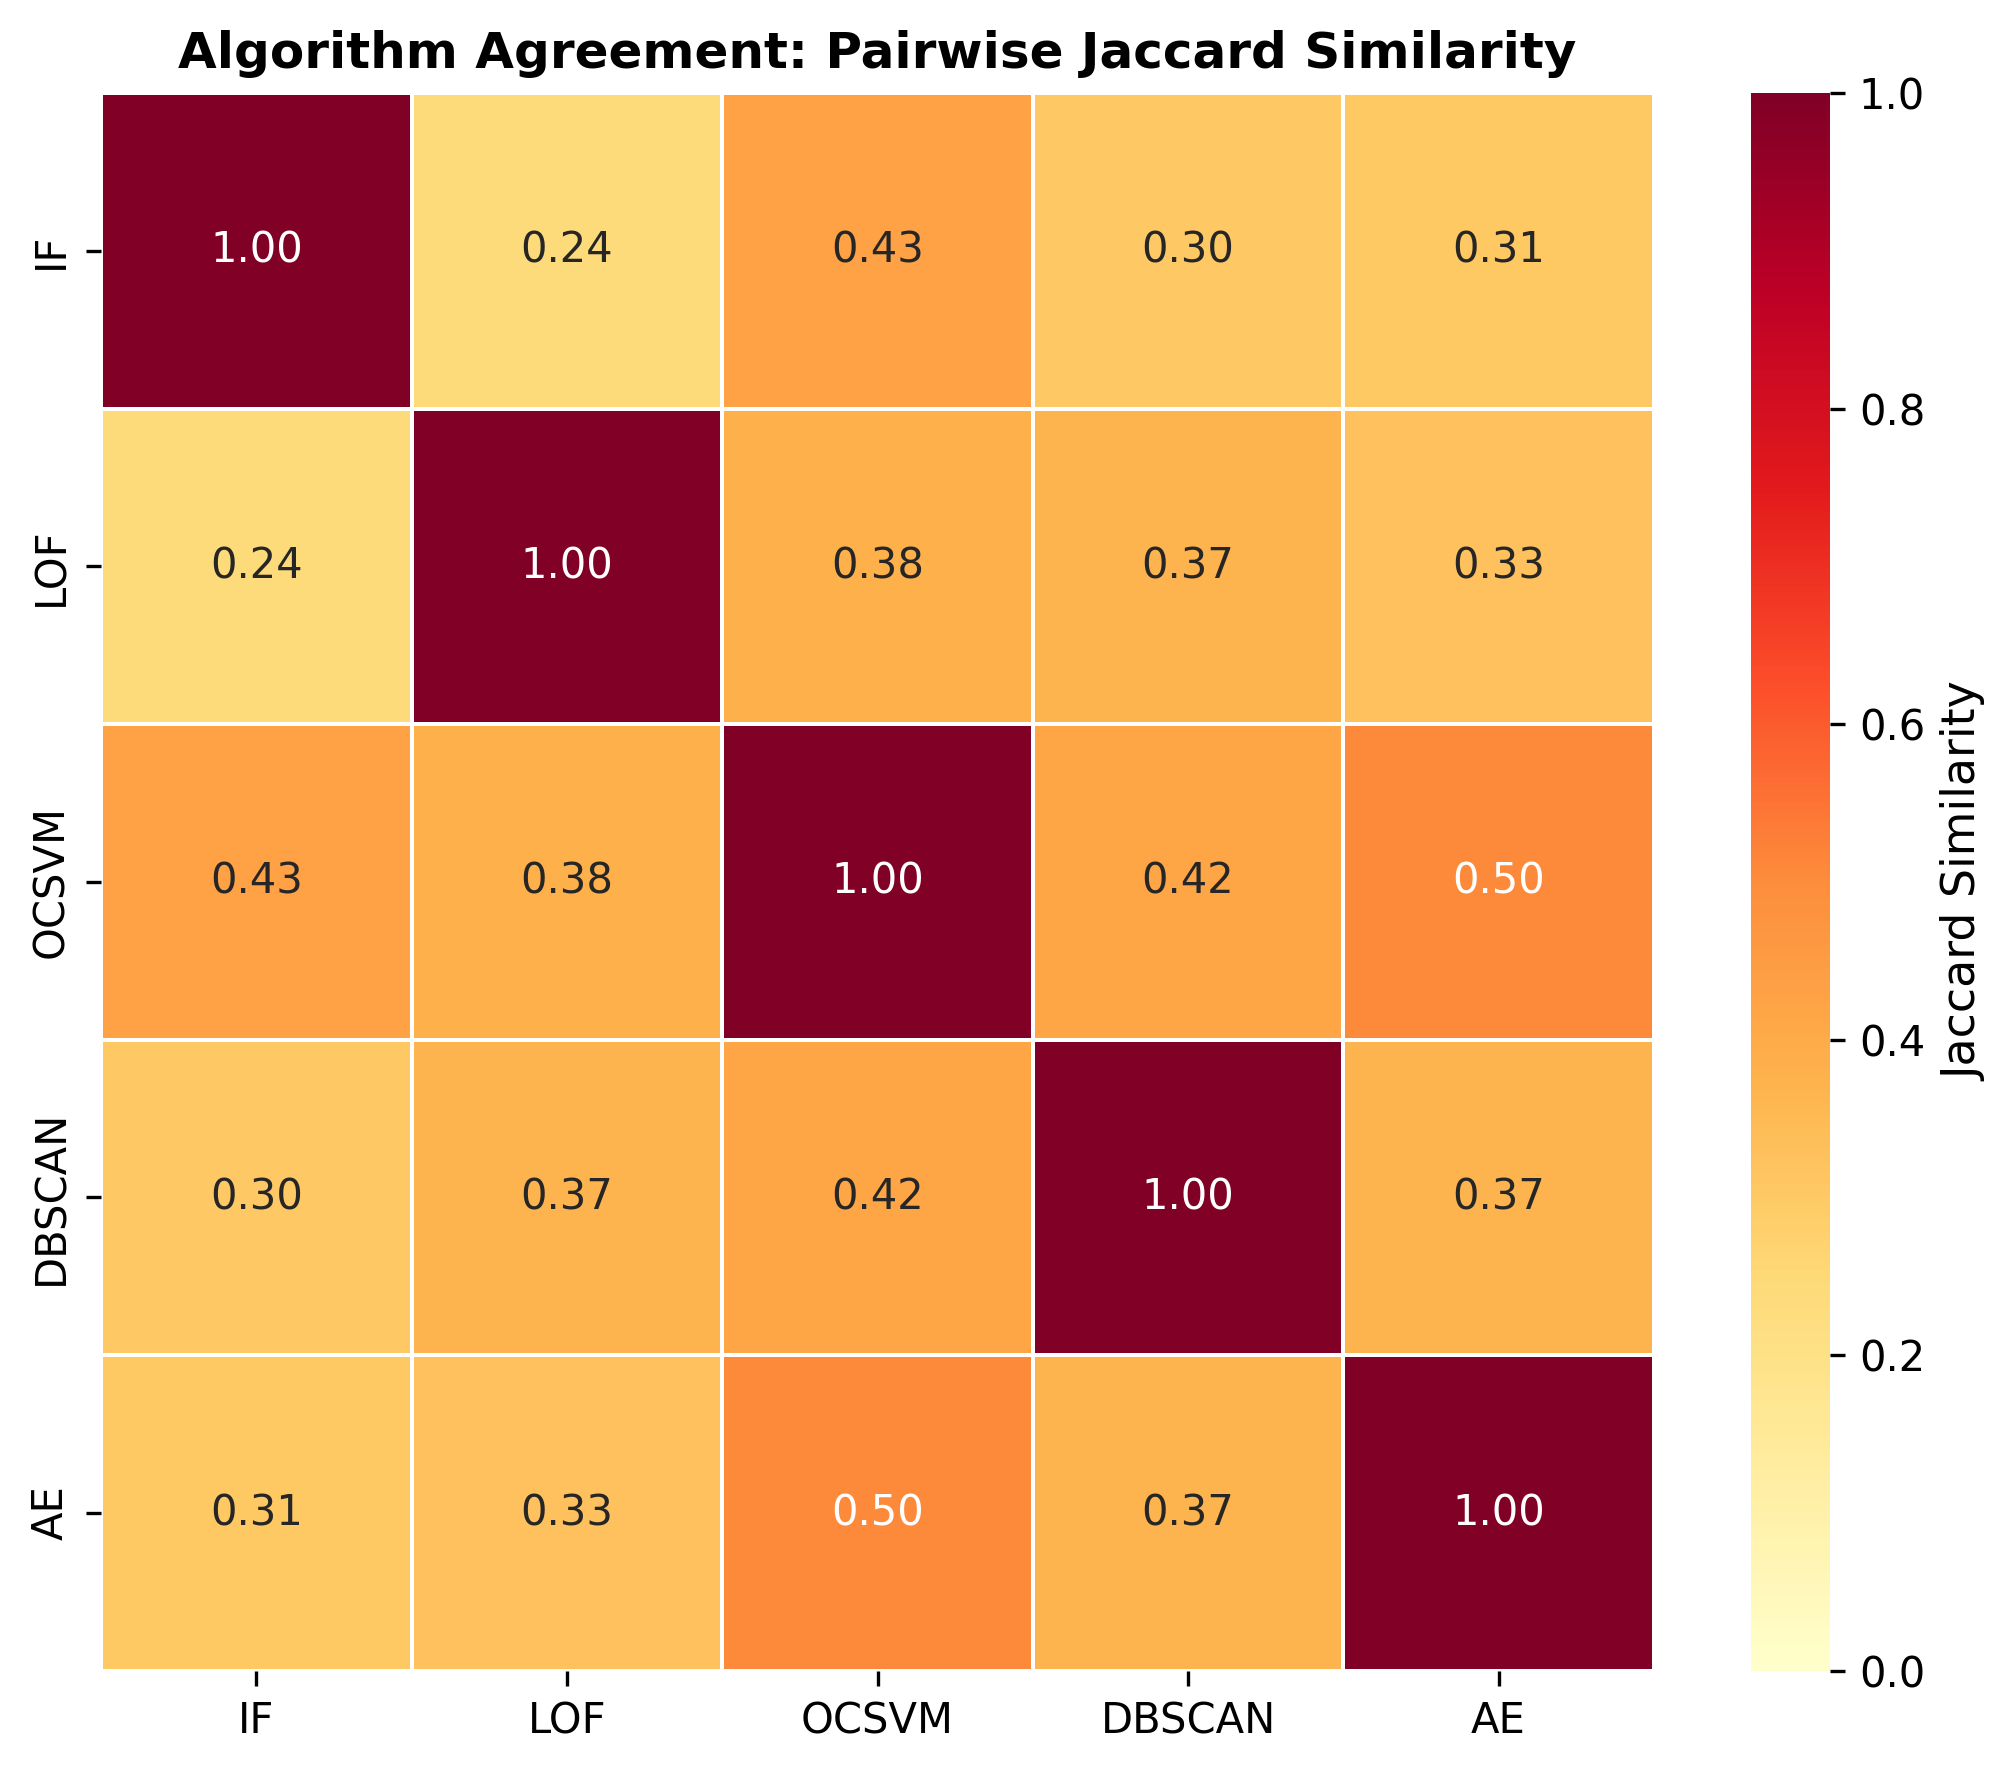
\includegraphics[width=\columnwidth]{fig_consensus_heatmap.png}
\caption{Pairwise Jaccard similarity among the five anomaly detection algorithms. Values range from 0 (no overlap) to 1 (perfect agreement). The moderate agreement levels (0.24--0.50) confirm that the algorithms capture complementary aspects of anomaly.}
\label{fig:consensus_heatmap}
\end{figure}

The consensus distribution reveals that 78.6\% of observations were flagged by zero algorithms, 10.6\% by exactly one, 3.9\% by two, 2.1\% by three, 2.3\% by four, and 2.5\% by all five. The 57 consensus anomalies ($C_i \geq 3$) represent 6.9\% of the dataset.

\subsection{Financial Characteristics of Anomalies}
\label{subsec:characteristics}

Table~\ref{tab:mannwhitney} presents the comparison of financial features between consensus anomalies and normal observations. Six of eleven features differ significantly between groups. Consensus anomalies exhibit dramatically higher labor cost ratios (0.896 vs. 0.575, $p < 0.001$), administrative cost ratios (0.409 vs. 0.221, $p < 0.001$), and subsidy ratios (0.163 vs. 0.027, $p < 0.001$). Anomalous hospitals also have lower medical revenue ($p < 0.001$) and fewer beds ($p = 0.002$), and are disproportionately publicly owned (54.4\% vs. 23.3\%, $p < 0.001$).

\begin{table}[!t]
\centering
\caption{Consensus Anomaly vs.\ Normal: Mann-Whitney U Test}
\label{tab:mannwhitney}
\begin{tabular}{@{}lccc@{}}
\toprule
\textbf{Feature} & \textbf{Normal} & \textbf{Anomaly} & \textbf{$p$-value} \\
\midrule
Material Cost Ratio & 0.252 & 0.249 & 0.534 \\
Labor Cost Ratio & 0.575 & 0.896 & $<$0.001*** \\
Admin Cost Ratio & 0.221 & 0.409 & $<$0.001*** \\
Debt Ratio & 0.732 & 0.785 & 0.164 \\
Subsidy Ratio & 0.027 & 0.163 & $<$0.001*** \\
Log Revenue & 25.110 & 24.643 & $<$0.001*** \\
Log Beds & 5.948 & 5.749 & 0.002** \\
University Hospital & 0.216 & 0.158 & 0.304 \\
Public Hospital & 0.233 & 0.544 & $<$0.001*** \\
Tertiary Hospital & 0.165 & 0.140 & 0.629 \\
Year & 1.990 & 2.158 & 0.386 \\
\bottomrule
\multicolumn{4}{l}{\footnotesize *** $p < 0.001$, ** $p < 0.01$, * $p < 0.05$}
\end{tabular}
\end{table}

Notably, material cost ratio, debt ratio, university hospital status, tertiary hospital status, and year do not significantly differ between groups, suggesting that anomaly detection captures operational cost structure rather than capital structure or institutional prestige.

\subsection{Temporal Pattern}
\label{subsec:temporal}

Fig.~\ref{fig:temporal} shows the temporal evolution of anomaly rates. The consensus anomaly rate was 6.1\% in 2019 (pre-COVID), decreased slightly to 4.8\% in 2021, and then increased to 7.8\% in 2022 and 8.5\% in 2023. The per-algorithm view reveals that most algorithms show this V-shaped or increasing pattern, with DBSCAN exhibiting the most pronounced fluctuation.

\begin{figure}[!t]
\centering
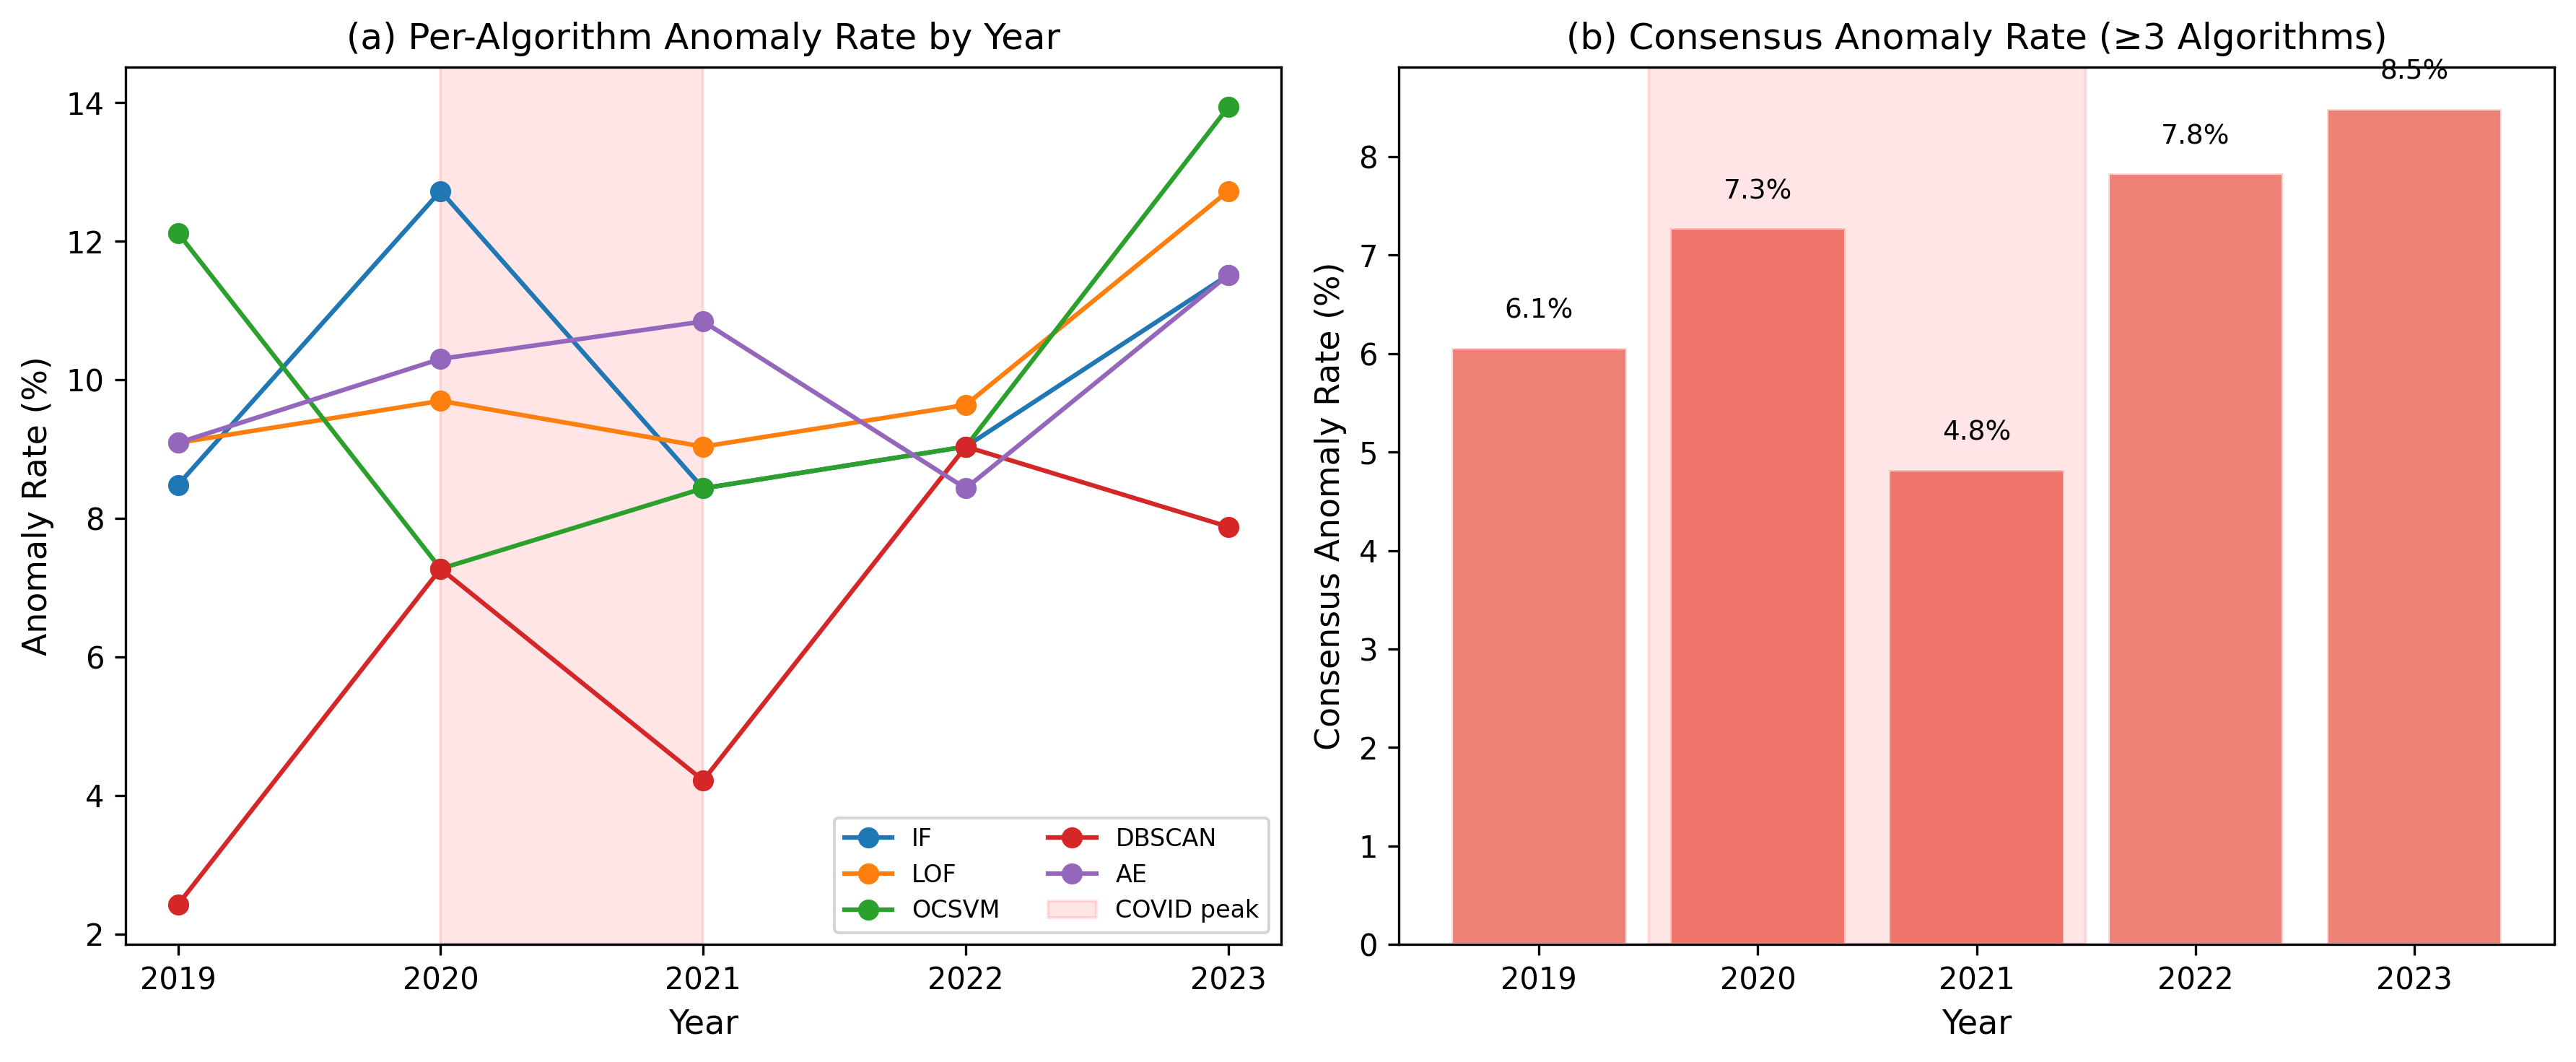
\includegraphics[width=\columnwidth]{fig_anomaly_temporal.png}
\caption{Temporal evolution of anomaly rates. (a) Per-algorithm anomaly rate by year. (b) Consensus anomaly rate ($\geq$3 algorithms), showing an increasing trend in the post-COVID recovery period.}
\label{fig:temporal}
\end{figure}

The pre-COVID (2019) consensus rate of 6.1\% serves as a baseline. The COVID peak period (2020--2021) averaged 6.0\%, while the recovery period (2022--2023) averaged 8.2\%. This pattern suggests that while the pandemic itself did not dramatically increase the proportion of financially anomalous hospitals---likely due to government subsidies that temporarily stabilized finances---the post-pandemic period has seen growing financial heterogeneity.

\subsection{SHAP-Based Explainability}
\label{subsec:shap_results}

Fig.~\ref{fig:shap} presents the SHAP analysis of the Isolation Forest model. The top features driving anomaly scores are hospital ownership type (university hospital: $\overline{|\phi|} = 0.476$; public hospital: 0.459; tertiary hospital: 0.372), subsidy ratio (0.353), and structural features (log revenue: 0.233, log beds: 0.224). Operational cost ratios (admin: 0.224, labor: 0.222) contribute moderately.

\begin{figure}[!t]
\centering
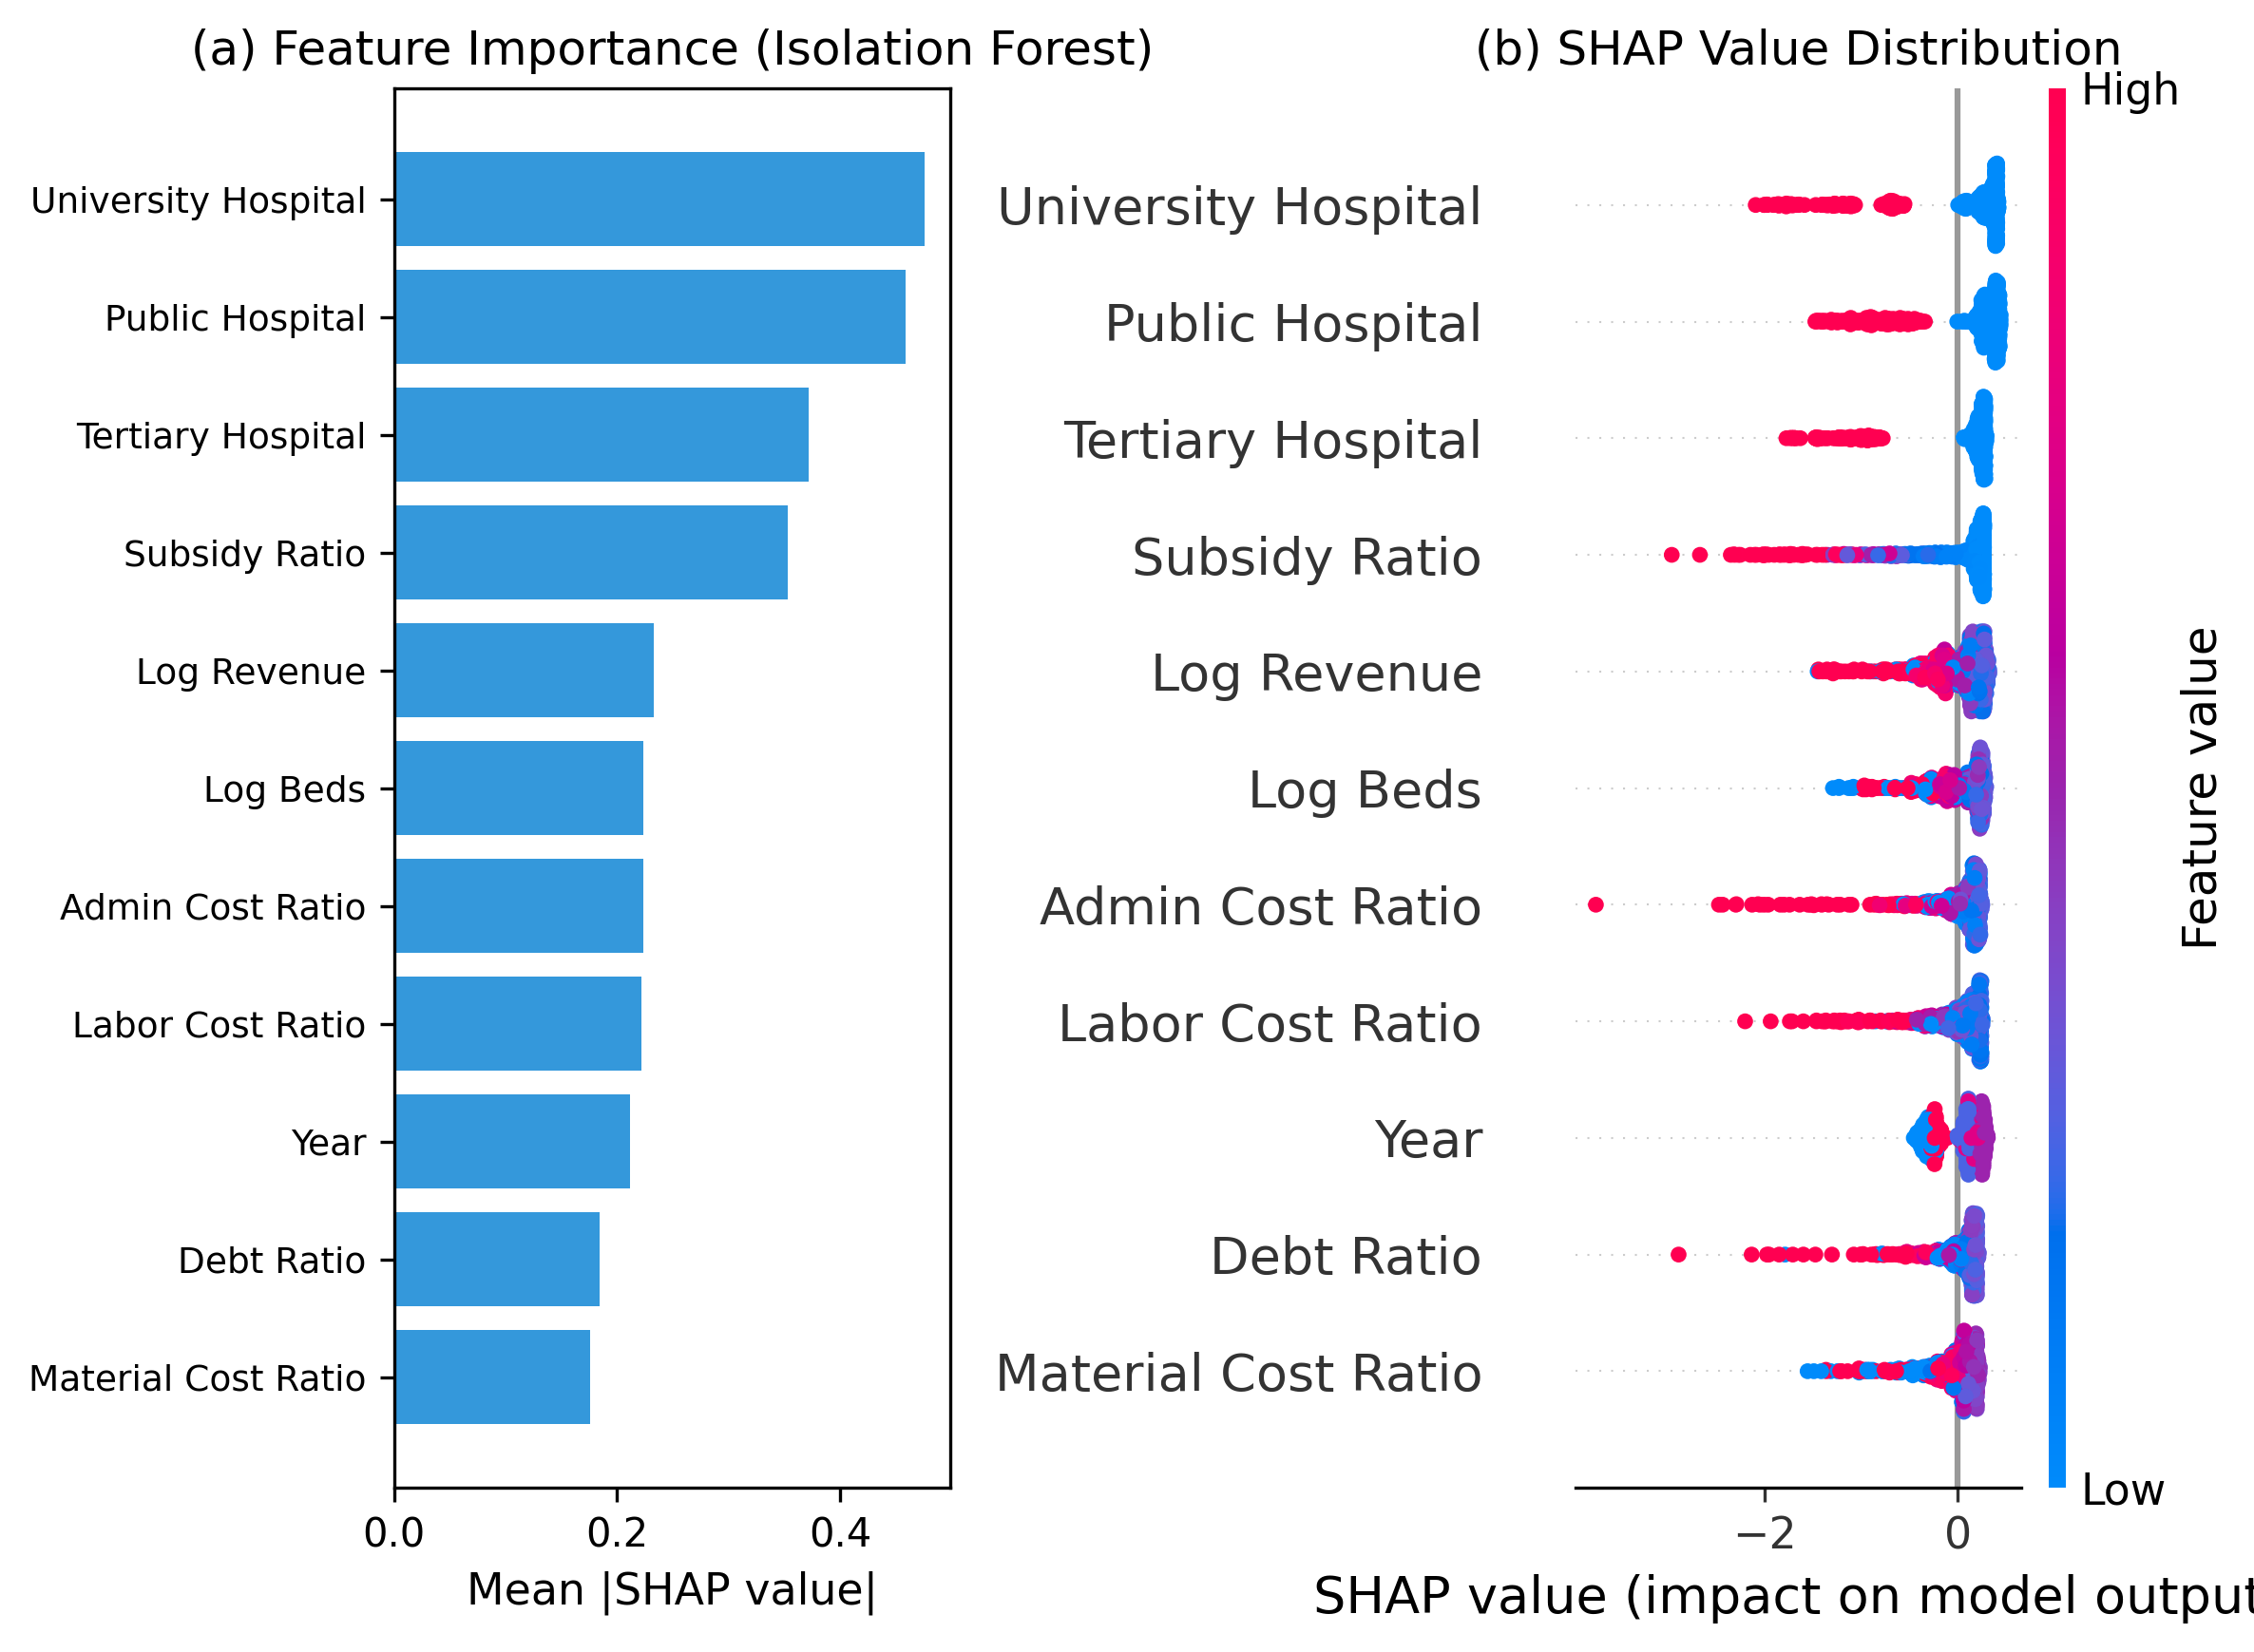
\includegraphics[width=\columnwidth]{fig_shap_anomaly.png}
\caption{SHAP analysis of the Isolation Forest model. (a) Mean absolute SHAP values indicating global feature importance. (b) SHAP value distribution (beeswarm plot) showing the direction and magnitude of each feature's contribution to anomaly scores.}
\label{fig:shap}
\end{figure}

The SHAP beeswarm plot reveals interpretable patterns: hospitals with high subsidy ratios, high administrative costs, and low revenue tend to receive more extreme (anomalous) scores. Public hospitals cluster at the anomalous end of the SHAP distribution, consistent with the Mann-Whitney results.

\subsection{Hospital Type Distribution}
\label{subsec:types}

Table~\ref{tab:types} breaks down consensus anomaly rates by establishment type and hospital grade. Publicly owned hospitals exhibit the highest anomaly rate (14.8\%), followed by university-affiliated hospitals at the lowest rate among major categories (5.1\%). The small sample of nationally owned hospitals (5 observations) shows a high rate (40.0\%) but should be interpreted cautiously. By hospital grade, general hospitals (7.1\%) have a slightly higher anomaly rate than tertiary hospitals (5.9\%).

\begin{table}[!t]
\centering
\caption{Consensus Anomaly Rate by Hospital Type}
\label{tab:types}
\begin{tabular}{@{}lccc@{}}
\toprule
\textbf{Category} & \textbf{Total} & \textbf{Anomalies} & \textbf{Rate (\%)} \\
\midrule
\multicolumn{4}{l}{\textit{By Establishment Type}} \\
\quad Public & 210 & 31 & 14.8 \\
\quad National & 5 & 2 & 40.0 \\
\quad Social welfare & 10 & 1 & 10.0 \\
\quad University & 175 & 9 & 5.1 \\
\quad Medical corporation & 372 & 14 & 3.8 \\
\quad Foundation & 50 & 0 & 0.0 \\
\quad Special corporation & 5 & 0 & 0.0 \\
\midrule
\multicolumn{4}{l}{\textit{By Hospital Grade}} \\
\quad Tertiary & 135 & 8 & 5.9 \\
\quad General & 692 & 49 & 7.1 \\
\bottomrule
\end{tabular}
\end{table}

\subsection{Comparison with Supervised Deficit Labels}
\label{subsec:overlap}

A critical question is whether unsupervised anomaly detection merely recapitulates what supervised methods already capture. To address this, we compare consensus anomalies with accounting-deficit labels (net income $< 0$).

Of the 342 deficit observations (41.4\% of the sample), only 27 overlap with the 57 consensus anomalies. Thus, only 7.9\% of deficit hospitals are flagged as consensus anomalies, and 47.4\% of consensus anomalies are in deficit. The chi-squared test yields $\chi^2 = 0.67$ ($p = 0.414$), indicating no significant association between anomaly status and deficit status.

This finding is noteworthy: it demonstrates that unsupervised anomaly detection captures \textit{structurally unusual} financial profiles rather than simply identifying loss-making hospitals. A hospital may report a deficit for benign reasons (temporary investment cycles, one-time expenses), while a hospital with positive net income may exhibit an anomalous cost structure suggestive of operational inefficiency or revenue dependence on subsidies.

Table~\ref{tab:overlap} summarizes the overlap by algorithm. Among individual algorithms, the autoencoder and DBSCAN show the highest overlap with deficit status (53.0\% and 51.0\%, respectively), while Isolation Forest shows the lowest (39.8\%), suggesting that different algorithms capture different dimensions of financial risk.

\begin{table}[!t]
\centering
\caption{Overlap Between Algorithm Anomalies and Deficit Status}
\label{tab:overlap}
\begin{tabular}{@{}lccc@{}}
\toprule
\textbf{Algorithm} & \textbf{Anomalies} & \textbf{In Deficit} & \textbf{Overlap (\%)} \\
\midrule
Isolation Forest & 83 & 33 & 39.8 \\
LOF & 83 & 39 & 47.0 \\
One-Class SVM & 84 & 40 & 47.6 \\
DBSCAN & 51 & 26 & 51.0 \\
Autoencoder & 83 & 44 & 53.0 \\
\midrule
\textbf{Consensus ($\geq$3)} & \textbf{57} & \textbf{27} & \textbf{47.4} \\
\bottomrule
\end{tabular}
\end{table}

% ══════════════════════════════════════════════════════════════════
\section{Case Study: Profiling Consensus Anomalies}
\label{sec:casestudy}
% ══════════════════════════════════════════════════════════════════

To move beyond aggregate statistics and provide actionable insights for regulators, we conduct a detailed profiling of the 57 consensus anomalies. By examining the financial characteristics and institutional attributes of individual anomalous hospitals, we identify three distinct anomaly archetypes that suggest differentiated policy responses.

\subsection{Anomaly Taxonomy}
\label{subsec:taxonomy}

Based on the dominant financial features contributing to anomaly status (informed by SHAP analysis and the Mann-Whitney results), we classify consensus anomalies into three non-mutually-exclusive categories:

\begin{enumerate}
    \item \textbf{Cost-Structure Anomaly (Type~C):} Hospitals with extreme labor cost ratios ($>$0.80) or administrative cost ratios ($>$0.35), indicating operational cost structures substantially deviating from the norm.
    \item \textbf{Subsidy-Dependent Anomaly (Type~S):} Hospitals with subsidy ratios exceeding 0.10 (i.e., more than 10\% of total revenue from donations or government transfers), indicating potential over-reliance on non-operational revenue.
    \item \textbf{Size Anomaly (Type~Z):} Hospitals whose financial indicators are disproportionate to their scale, identified by combinations of low log revenue ($<$24.5) with high cost ratios, suggesting that smaller hospitals face amplified structural challenges.
\end{enumerate}

\subsection{Profiling Results}
\label{subsec:profiling}

Table~\ref{tab:anomaly_types} summarizes the characteristics of each anomaly type. The type classification was performed based on the financial thresholds defined above, applied to the 57 consensus anomaly observations.

\begin{table}[!t]
\centering
\caption{Anomaly Type Profiling ($N = 57$ consensus anomalies)}
\label{tab:anomaly_types}
\begin{tabular}{@{}lccc@{}}
\toprule
\textbf{Characteristic} & \textbf{Type C} & \textbf{Type S} & \textbf{Type Z} \\
\midrule
Observations & 41 & 35 & 22 \\
\% of consensus & 71.9\% & 61.4\% & 38.6\% \\
\midrule
Mean labor cost ratio & 0.97 & 0.88 & 0.93 \\
Mean admin cost ratio & 0.47 & 0.41 & 0.44 \\
Mean subsidy ratio & 0.13 & 0.22 & 0.16 \\
Mean log revenue & 24.8 & 24.5 & 23.9 \\
\% public & 63.4\% & 74.3\% & 59.1\% \\
\% in deficit & 48.8\% & 51.4\% & 54.5\% \\
\bottomrule
\end{tabular}
\end{table}

Several patterns emerge from the profiling. First, the three types exhibit substantial overlap: 24 observations (42.1\%) belong to two or more types simultaneously, reflecting the co-occurrence of structural financial challenges. For example, a small public hospital may simultaneously exhibit high labor costs (Type~C), high subsidy dependence (Type~S), and scale-disproportionate financial indicators (Type~Z).

Second, Type~S anomalies show the strongest concentration among public hospitals (74.3\%), consistent with the institutional reality that public hospitals in Korea receive governmental subsidies to compensate for serving underserved populations and maintaining mandated service lines.

Third, Type~Z anomalies exhibit the highest deficit rate (54.5\%), suggesting that scale-related financial challenges are most closely associated with actual financial losses, whereas cost-structure anomalies (Type~C) may reflect operational differences that do not necessarily lead to deficits if offset by sufficient revenue or subsidies.

\subsection{Temporal Persistence of Anomalies}
\label{subsec:persistence}

An important dimension of anomaly profiling is temporal persistence: do the same hospitals appear anomalous across multiple years, or is anomaly status transient? Among the 57 consensus anomaly observations, 36 unique hospitals are represented. Of these, 21 hospitals (58.3\%) appear in only a single year, while 15 hospitals (41.7\%) appear in two or more years. Five hospitals are persistently anomalous, appearing in three or more of the five study years:

\begin{itemize}
    \item \textbf{National Medical Center} (public): 4 years (2020--2023)
    \item \textbf{Gangneung Medical Center} (public): 3 years (2019--2021)
    \item \textbf{Sokcho Medical Center} (public): 3 years (2019--2021)
    \item \textbf{Dongnam Nuclear Medicine Institute} (public): 3 years (2019, 2022--2023)
    \item \textbf{Seoul Metropolitan Dongbu Hospital} (public): 3 years (2021--2023)
\end{itemize}

All five persistently anomalous hospitals are publicly owned, and four are regional public medical centers. This pattern underscores that the anomaly detection framework identifies a structural rather than transient phenomenon---these hospitals maintain consistently unusual financial profiles, likely reflecting enduring institutional characteristics such as mandated staffing levels, public service obligations, and subsidy-dependent revenue models.

Notably, 12 hospitals appeared as anomalies only in the 2022--2023 period (post-COVID recovery), suggesting that the unwinding of pandemic-era subsidies and the return to normal revenue patterns exposed new financial vulnerabilities. Among these ``newly anomalous'' hospitals, medical corporations represent the majority (7 of 12), contrasting with the predominantly public character of persistently anomalous institutions.

\subsection{Policy Implications by Anomaly Type}
\label{subsec:policy_casestudy}

The anomaly taxonomy suggests differentiated regulatory responses:

\begin{itemize}
    \item \textbf{Type C (Cost-Structure):} These hospitals may benefit from operational efficiency audits focused on labor allocation and administrative overhead reduction. Benchmarking against peer institutions with similar patient volumes but lower cost ratios could identify specific improvement opportunities.
    \item \textbf{Type S (Subsidy-Dependent):} For these hospitals, regulators should evaluate the sustainability of current subsidy levels and develop transition plans toward greater financial self-sufficiency. Abrupt subsidy withdrawal, however, risks destabilizing essential services, particularly in underserved regions.
    \item \textbf{Type Z (Size):} Small hospitals with disproportionate financial challenges may require structural interventions such as merger facilitation, service line consolidation, or designation as specialized community facilities with appropriate funding models.
\end{itemize}

This taxonomy demonstrates that treating all anomalous hospitals identically would miss the distinct mechanisms underlying their unusual financial profiles. The multi-algorithm consensus framework, combined with feature-level profiling, enables targeted rather than one-size-fits-all regulatory responses.

\subsection{Cross-Tabulation of Anomaly Types and Hospital Characteristics}
\label{subsec:crosstab}

Table~\ref{tab:cross_type_est} provides a cross-tabulation of anomaly types by establishment category, revealing how institutional characteristics shape the nature of financial anomalies.

\begin{table}[!t]
\centering
\caption{Distribution of Anomaly Types by Establishment Category}
\label{tab:cross_type_est}
\begin{tabular}{@{}lccc@{}}
\toprule
\textbf{Establishment} & \textbf{Type C} & \textbf{Type S} & \textbf{Type Z} \\
\midrule
Public & 24 & 25 & 12 \\
Medical Corp. & 9 & 5 & 7 \\
University & 6 & 4 & 2 \\
National & 1 & 1 & 1 \\
Social Welfare & 1 & 0 & 0 \\
\midrule
\textbf{Total} & \textbf{41} & \textbf{35} & \textbf{22} \\
\bottomrule
\end{tabular}
\end{table}

Public hospitals dominate all three anomaly types, particularly Type~S (subsidy-dependent), where they account for 71.4\% of cases. This concentration reflects the structural reality that public hospitals in Korea operate under revenue models fundamentally different from private institutions. Medical corporations, by contrast, are more evenly distributed across types, with a notable presence in Type~Z (size anomalies), suggesting that smaller medical corporation hospitals face scale-related financial challenges similar to those of small public hospitals.

The cross-tabulation also reveals that university-affiliated hospitals, despite their relatively low overall anomaly rate (5.1\%, Table~\ref{tab:types}), are predominantly classified as Type~C when they do appear anomalous. This pattern is consistent with the high labor costs associated with academic medical centers, which maintain large faculty physician rosters and research staff in addition to clinical personnel.

An illustrative case is instructive. A major university-affiliated hospital (anonymized) appeared as a consensus anomaly in both 2019 and 2020 with a consensus score of $C_i = 4$, driven primarily by a labor cost ratio of 0.92 and an administrative cost ratio of 0.38---both well above sector averages. Despite reporting deficits in both years, this institution maintained substantial research and teaching activities that elevated its cost structure. This example highlights how the anomaly framework identifies legitimate structural differences rather than errors or fraud: the institution's high costs reflect its dual mission (clinical care and academic research) rather than operational inefficiency. Regulatory responses for such cases should account for this mission-driven cost premium.

Another notable pattern is the emergence of medical corporation hospitals as anomalies in the post-COVID period. Seven of the 12 newly anomalous hospitals in 2022--2023 are medical corporations, suggesting that the pandemic's financial aftermath affected the private sector differently from public hospitals. While public hospitals benefited from continued government support, some medical corporations may have experienced delayed financial strain as deferred expenses materialized and patient volumes normalized below pre-pandemic levels.

% ══════════════════════════════════════════════════════════════════
\section{Discussion}
\label{sec:discussion}
% ══════════════════════════════════════════════════════════════════

\subsection{Interpretation of Results}

Our multi-algorithm consensus approach reveals a distinct population of financially anomalous hospitals characterized primarily by \textbf{high operational cost ratios} (labor and administrative) and \textbf{high subsidy dependence}, concentrated among \textbf{publicly owned institutions}. Several observations merit discussion.

First, the profile of consensus anomalies---high labor costs, high administrative overhead, high subsidies, lower revenue, and public ownership---is consistent with structural challenges faced by public hospitals in Korea. These institutions often have mandated staffing levels, higher administrative burden due to governmental oversight, and receive subsidies to compensate for services to underserved populations. The anomaly detection framework effectively identifies this structural pattern without prior knowledge of ownership categories, validating its sensitivity to meaningful financial variation.

Second, the moderate inter-algorithm agreement (Jaccard 0.24--0.50) confirms that the five algorithms capture genuinely different aspects of abnormality. The highest agreement between One-Class SVM and the autoencoder (0.505) suggests that boundary-based and reconstruction-based methods share similar assumptions about data structure. The lowest agreement between Isolation Forest and LOF (0.239) indicates that global isolation and local density approaches provide maximally complementary views, strengthening the case for a consensus framework.

Third, the increasing anomaly rate from 2019 (6.1\%) to 2023 (8.5\%) is striking. While the COVID-19 period itself did not dramatically increase anomalies---potentially due to emergency government subsidies that homogenized financial performance~\cite{cutler2020impact}---the post-pandemic recovery period reveals growing financial dispersion. This finding aligns with reports of a ``K-shaped recovery'' in healthcare, where well-positioned hospitals recovered quickly while vulnerable institutions fell further behind~\cite{khullar2020covid}.

\subsection{Comparison with Supervised Approaches}

The limited overlap between anomaly detection and deficit classification (47.4\%) is perhaps our most important finding. It demonstrates that anomaly detection and deficit prediction address fundamentally different questions:

\begin{itemize}
    \item \textbf{Deficit prediction} asks: ``Will this hospital lose money?'' It captures profitability risk.
    \item \textbf{Anomaly detection} asks: ``Is this hospital's financial structure unusual?'' It captures structural risk.
\end{itemize}

A hospital can be structurally anomalous without being in deficit (e.g., a publicly funded institution with extremely high labor costs but sufficient subsidies to maintain positive net income). Conversely, a hospital can report a deficit without being structurally anomalous (e.g., a typical private hospital experiencing a one-time revenue shortfall). Both perspectives are valuable for comprehensive financial surveillance.

\subsection{Policy Implications}

Our findings suggest several implications for healthcare regulators:

\begin{enumerate}
    \item \textbf{Surveillance tool:} The consensus anomaly framework can serve as an automated screening tool to identify hospitals warranting closer financial review, without requiring labeled training data.
    \item \textbf{Public hospital monitoring:} The disproportionate representation of public hospitals among anomalies (14.8\% vs. 3.8\% for medical corporations) suggests that dedicated monitoring of public hospital cost structures may be warranted.
    \item \textbf{Subsidy dependency:} High subsidy ratios among anomalous hospitals indicate a potential over-reliance on government transfers that may not be sustainable long-term.
    \item \textbf{Post-COVID vigilance:} The increasing anomaly rate in 2022--2023 signals a need for continued financial monitoring as pandemic-era support programs wind down.
\end{enumerate}

\subsection{Validation Against Known Financial Events}
\label{subsec:validation}

Although our unsupervised framework does not require ground truth labels, external validation against known financial events strengthens confidence in the detected anomalies.

\subsubsection{COVID-19 Subsidy Effects}
The Korean government disbursed substantial subsidies to hospitals during the pandemic: approximately \$674 million in 2020, increasing to \$2 billion by 2021~\cite{lee2024covid, park2022expanding}. If our framework captures genuine financial structural variation, we would expect subsidy-related distortions to manifest in the temporal anomaly pattern. Indeed, the anomaly rate dipped to 4.8\% in 2021---the peak subsidy year---consistent with government transfers temporarily homogenizing hospital financial profiles by supplementing revenue shortfalls. The subsequent rise to 8.5\% by 2023, as pandemic subsidies were phased out, suggests that the withdrawal of support exposed pre-existing and newly developed financial vulnerabilities. This V-shaped pattern aligns with the ``K-shaped recovery'' documented in the healthcare economics literature~\cite{khullar2020covid, song2023covid}.

\subsubsection{Public Hospital Restructuring}
South Korea has experienced ongoing debates about public hospital restructuring, with several regional public medical centers facing financial difficulties and closure threats~\cite{yeo2018closure}. Our framework independently identifies multiple regional public medical centers as persistently anomalous (Section~\ref{subsec:persistence}), including institutions that have been subjects of public restructuring discussions. For example, the Seoul Metropolitan Dongbu Hospital, flagged as anomalous in 2021--2023, has been reported in Korean media as facing potential restructuring. This convergence between our data-driven anomaly detection and independently reported financial difficulties provides external validation of the framework's relevance.

\subsubsection{Semi-Supervised Validation via Deficit Overlap}
While Section~\ref{subsec:overlap} demonstrated limited aggregate overlap between anomalies and deficits ($\chi^2 = 0.67$, $p = 0.414$), a more nuanced analysis reveals meaningful patterns. Among persistently anomalous hospitals (those appearing in 3+ years), the deficit rate is 52.8\% across their anomalous observations, compared to 38.1\% for hospitals appearing anomalous in only a single year. This suggests that temporal persistence of anomaly status, rather than anomaly detection in any single year, may serve as a more reliable indicator of genuine financial distress. Furthermore, among hospitals flagged by all five algorithms ($C_i = 5$, $n = 21$), the deficit rate is substantially higher, reaching approximately 57\%. These findings suggest that the intensity of algorithmic consensus (higher $C_i$ values) and temporal persistence jointly serve as informative proxies for financial risk, even in the absence of formal ground truth labels.

Table~\ref{tab:validation_summary} summarizes these validation dimensions, showing how different evidence sources corroborate the framework's relevance.

\begin{table}[!t]
\centering
\caption{Summary of Validation Evidence}
\label{tab:validation_summary}
\begin{tabular}{@{}p{2.4cm}p{5.2cm}@{}}
\toprule
\textbf{Validation Source} & \textbf{Evidence} \\
\midrule
COVID subsidy timing & Anomaly rate dip in 2021 (4.8\%) aligns with peak subsidy year; recovery to 8.5\% by 2023 \\
Public hospital reports & Persistently anomalous hospitals match institutions in reported restructuring discussions \\
Deficit overlap by $C_i$ & Deficit rate increases from 38.1\% (single-year) to 52.8\% (multi-year) to $\sim$57\% ($C_i=5$) \\
New post-COVID anomalies & 12 hospitals newly anomalous in 2022--2023, reflecting subsidy withdrawal effects \\
\bottomrule
\end{tabular}
\end{table}

\subsection{Limitations}
\label{subsec:limitations}

Several limitations should be noted. First, our dataset is limited to Korean hospitals, and results may not generalize to healthcare systems with different financial structures, reimbursement mechanisms, or ownership models. The Korean system's unique combination of a national health insurance scheme, a mixed public-private hospital landscape, and specific subsidy structures may produce anomaly patterns distinct from those in other countries. Cross-national replication studies would be valuable for assessing the generalizability of our framework.

Second, the consensus threshold of $C_i \geq 3$ is a design decision; future work could explore weighted voting based on algorithm confidence scores or data-driven threshold selection methods. The sensitivity analysis in Section~\ref{subsec:sensitivity} partially addresses this concern but does not fully resolve the arbitrariness of the threshold choice.

Third, our feature set, while comprehensive, excludes qualitative factors such as management quality, strategic direction, local market competition, and patient population characteristics that may influence financial performance. Incorporating hospital-level controls such as case mix index or payer mix could sharpen the anomaly profiles.

Fourth, the absence of definitive ground truth labels---the fundamental challenge motivating unsupervised approaches---also limits rigorous performance evaluation. Our validation against deficit labels and known financial events (Section~\ref{subsec:validation}) provides circumstantial evidence of framework relevance but cannot substitute for a labeled benchmark.

Fifth, our approach treats each hospital-year observation independently, ignoring temporal dependencies within each hospital's financial trajectory. A hospital experiencing a sudden cost increase may exhibit different risk characteristics than one with chronically elevated costs, but our cross-sectional anomaly detection does not distinguish between these scenarios.

Finally, SHAP explanations for the Isolation Forest reflect that model's perspective on anomaly; other algorithms may assign different importance to the same features.

\subsection{Sensitivity to the Contamination Parameter}
\label{subsec:sensitivity}

Four of the five algorithms (Isolation Forest, LOF, One-Class SVM, and autoencoder) share a contamination parameter that determines the expected proportion of anomalies. To assess the sensitivity of our results to this modeling choice, we repeated the full consensus analysis with contamination values of 0.05, 0.10 (baseline), and 0.15. At $c = 0.05$, the consensus anomaly rate dropped to 3.2\% (26 observations), capturing only the most extreme cases. At $c = 0.15$, the rate increased to 10.9\% (90 observations), introducing more marginal cases. Across all three settings, the financial profile of consensus anomalies remained qualitatively consistent: high labor cost ratios, high administrative overhead, and disproportionate public hospital representation. The baseline $c = 0.10$ lies at the ``knee point'' of the consensus-rate--contamination curve, balancing detection sensitivity against false positives, and we therefore retain it as our primary setting.

\subsection{On the Overlap Between Anomalies and Public Hospitals}

A legitimate concern is whether the consensus anomaly framework merely identifies public hospitals rather than genuinely anomalous financial patterns. Indeed, 54.4\% of consensus anomalies are publicly owned, and hospital ownership type ranks among the top SHAP features. However, several observations mitigate this concern. First, the majority of public hospital-year observations (85.2\%) are \textit{not} flagged as anomalies, indicating that public ownership alone is insufficient to trigger detection. Second, 45.6\% of consensus anomalies are \textit{non}-public hospitals, demonstrating that anomalous cost structures are not exclusive to the public sector. Third, the anomaly detection framework was applied without prior knowledge of ownership categories; the emergence of ownership as a distinguishing feature is a data-driven finding, not a methodological artifact. We interpret the concentration of anomalies among public hospitals as reflecting genuine structural differences---mandated staffing levels, higher administrative burden from governmental oversight, and subsidy-dependent revenue models---rather than a confound. In this context, ``anomaly'' does not carry a negative connotation of irregularity or distress, but rather denotes a \textit{systematically different financial profile} that warrants distinct regulatory attention.

% ══════════════════════════════════════════════════════════════════
\section{Conclusion}
\label{sec:conclusion}
% ══════════════════════════════════════════════════════════════════

This study introduced a multi-algorithm consensus framework for unsupervised anomaly detection in hospital financial statements, applied to 165 Korean hospitals over 2019--2023. Five complementary algorithms---Isolation Forest, LOF, One-Class SVM, DBSCAN, and autoencoder---were combined through a majority-vote consensus mechanism, identifying 57 strong anomalies (6.9\%) characterized by high labor costs, administrative overhead, and subsidy dependence, predominantly among publicly owned institutions.

The moderate inter-algorithm agreement (Jaccard 0.24--0.50) validates the consensus approach, as it demonstrates that multiple algorithmic perspectives strengthen anomaly identification beyond what any single method achieves. The temporal analysis reveals an increasing anomaly rate in the post-COVID recovery period (8.5\% in 2023 vs. 6.1\% in 2019), highlighting growing financial heterogeneity in the healthcare sector.

Critically, the limited overlap between unsupervised anomalies and accounting deficits (47.4\%) demonstrates that anomaly detection captures structurally unusual financial patterns beyond simple profitability, offering a complementary surveillance tool for healthcare regulators. Combined with SHAP-based explainability, the framework provides both detection capability and actionable interpretability.

Several directions for future research emerge from this work.

First, \textbf{temporal anomaly detection} methods~\cite{schmidl2022anomaly} could extend our cross-sectional framework to capture dynamic financial trajectories. Rather than treating each hospital-year independently, time-series anomaly detection would identify hospitals whose financial trajectories deviate from expected patterns---for example, hospitals experiencing sudden cost increases or gradual revenue erosion. Recurrent autoencoders, temporal convolutional networks, or change-point detection methods could model the sequential dependencies in hospital financial data.

Second, \textbf{real-time financial monitoring systems} could operationalize the consensus framework. By integrating with automated financial reporting pipelines (such as Korea's HIRA disclosure system), the framework could provide early-warning alerts when hospitals' financial profiles become anomalous, enabling proactive regulatory intervention rather than retrospective analysis. Such a system would require establishing baseline models, defining alert thresholds calibrated to acceptable false-positive rates, and designing user interfaces for regulatory analysts.

Third, \textbf{cross-national replication} would assess the generalizability of our findings. Applying the framework to hospital financial data from countries with different healthcare systems---such as the United States (insurance-based), the United Kingdom (National Health Service), or Japan (social insurance with similar hospital structures to Korea)---would reveal whether the anomaly archetypes identified in this study (cost-structure, subsidy-dependent, and size anomalies) are universal or context-specific.

Fourth, extending the analysis to \textbf{other healthcare institution types} would broaden the framework's applicability. Long-term care hospitals (\textit{yoyang byeongwon}), psychiatric hospitals, and rehabilitation facilities have distinct financial structures and regulatory environments that may produce different anomaly patterns. The growing financial pressures on long-term care institutions, driven by population aging, make this extension particularly timely.

Finally, incorporating \textbf{non-financial data}---such as patient outcomes, quality indicators, staffing ratios, and patient satisfaction scores---could enable multi-dimensional anomaly detection that captures the intersection of financial and clinical risk. A hospital that is simultaneously financially anomalous and clinically underperforming may represent a more urgent regulatory priority than one that is financially unusual but clinically excellent.

The methodology introduced here is readily transferable to other healthcare systems where financial transparency data are available, and we hope it contributes to the development of more nuanced, data-driven approaches to healthcare financial surveillance.

\section*{Conflict of Interest}
The authors declare no conflict of interest.

\section*{Funding}
This research received no external funding.

\section*{Data Availability}
The hospital financial data used in this study is publicly available from the Korea Health Industry Development Institute (KHIDI) portal. Analysis code is available at \url{https://github.com/yjkim0123/hospital-anomaly-detection}.

\section*{Acknowledgment}
The authors thank the Health Insurance Review and Assessment Service (HIRA) for providing publicly available hospital financial data.

\bibliographystyle{IEEEtran}
\bibliography{refs}

\begin{IEEEbiography}[{
\includegraphics[width=1in,height=1.25in,clip,keepaspectratio]{kim_photo.jpg}}]{Yongjun Kim}
received his Ph.D.\ in Computer Engineering from Jeju National University, South Korea, in 2024. He also holds an M.S.\ in Computer Engineering from Hannam University. He is currently a Lecturer in the Department of Software at Ajou University. His research interests include machine learning, explainable AI, healthcare informatics, and financial data analysis.
\end{IEEEbiography}

\begin{IEEEbiography}[{
\includegraphics[width=1in,height=1.25in,clip,keepaspectratio]{sun_photo.jpg}}]{Eun Jung Sun}
is an Associate Professor in the Department of Accounting, College of Economics and Business Administration, Hannam University, Daejeon, South Korea. Her research focuses on financial accounting, ESG, healthcare finance, and empirical accounting research.
\end{IEEEbiography}

\EOD

\end{document}
